\documentclass{article}

\usepackage{graphicx}
\usepackage{tikz}
\usepackage{tikzsymbols}
\usetikzlibrary{calc,patterns,shapes.geometric}
\pagestyle{empty}
\usepackage[margin=0pt]{geometry}
\geometry{papersize={14in,12in}}

\def\centerarc[#1](#2)(#3:#4:#5){\draw[#1] ($(#2)+({#5*cos(#3)},{#5*sin(#3)})$) arc (#3:#4:#5);}

\begin{document}
	\begin{figure}
		\centering
		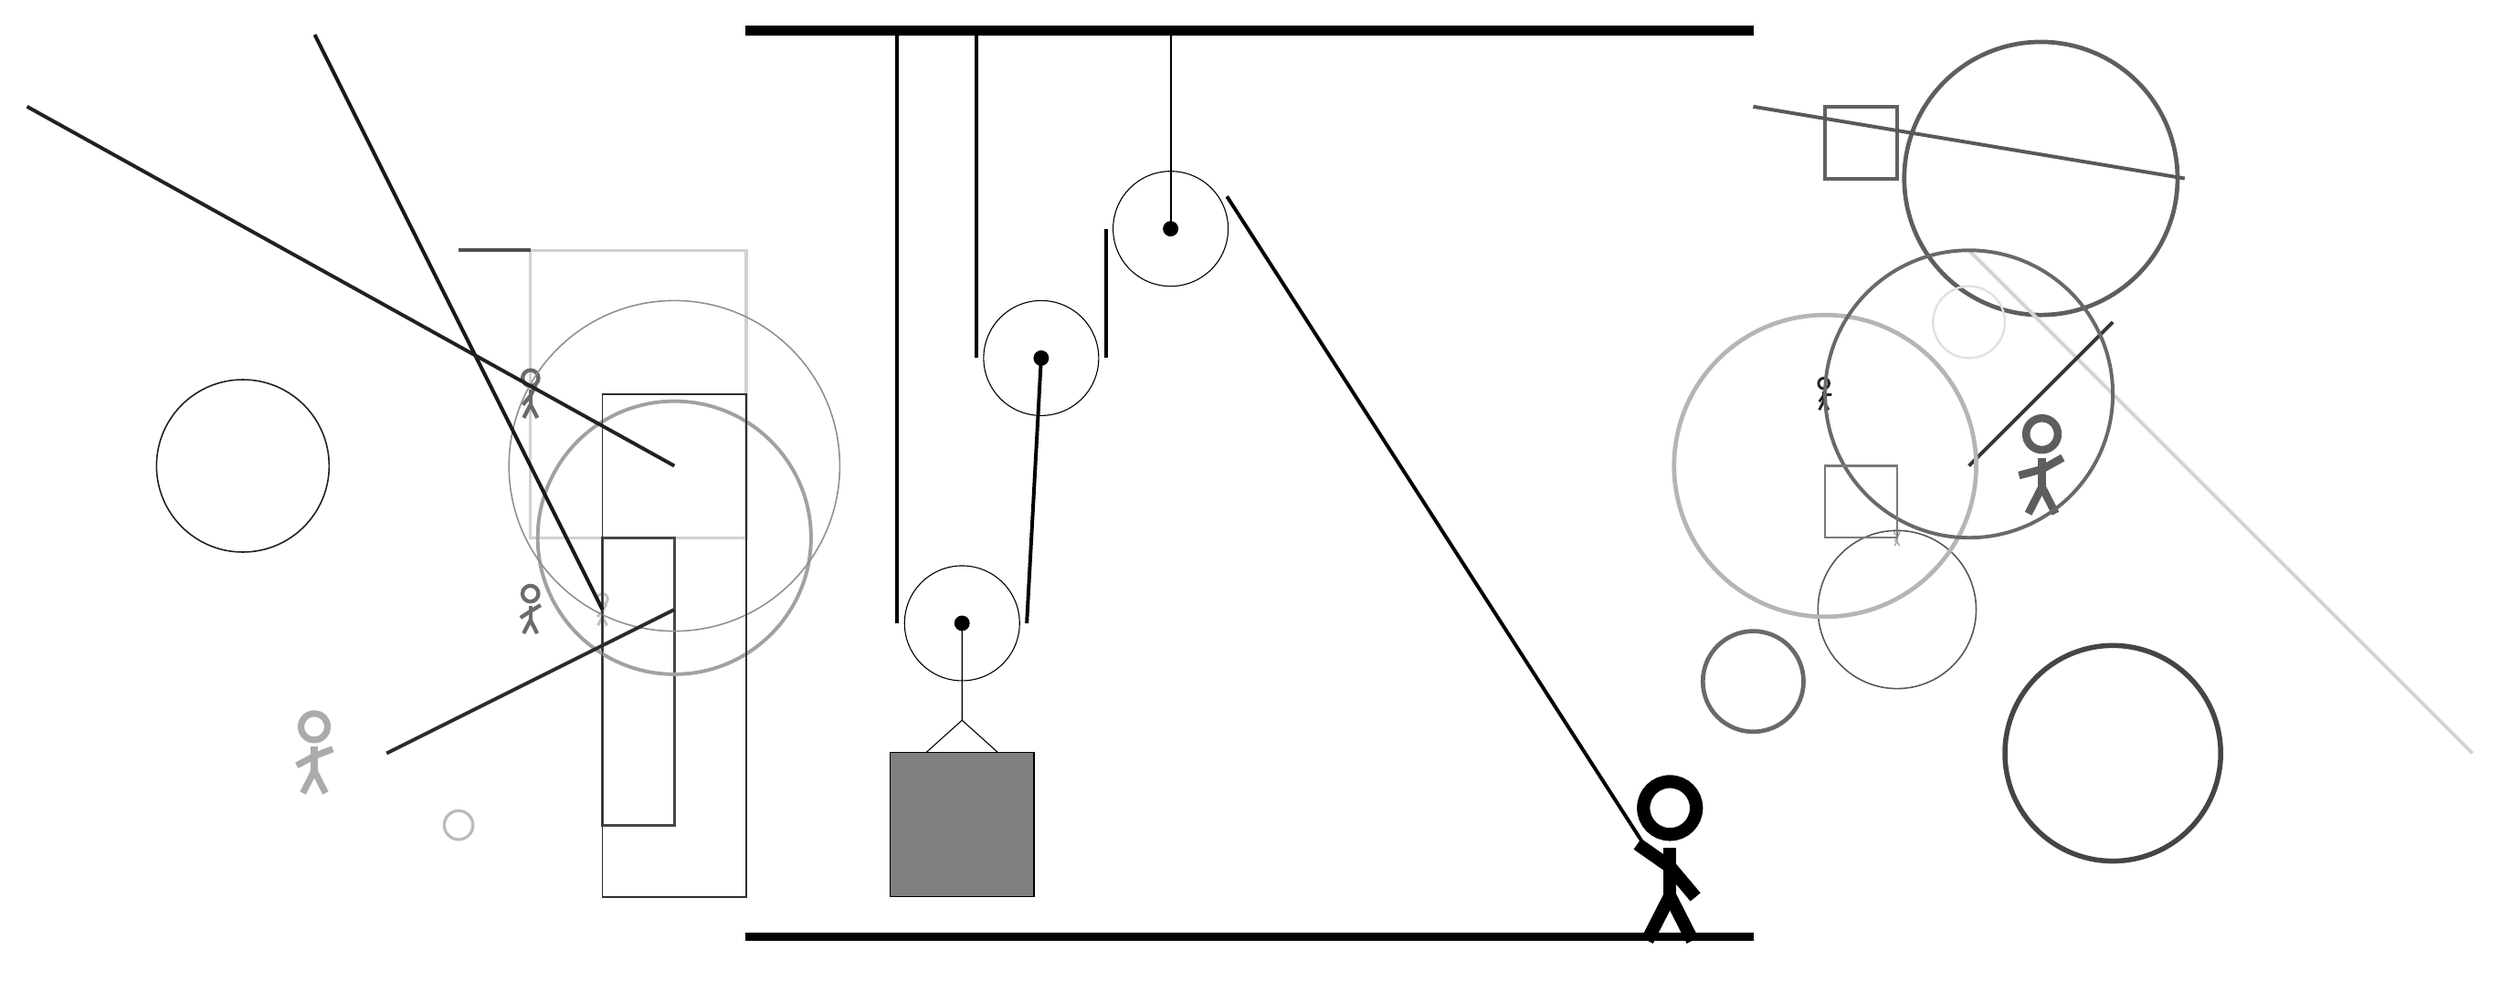
\begin{tikzpicture}
			%%%%% START %%%%%
			
			\draw[fill=black] (-2, 9) rectangle (12, 9.125);
			
			\draw[line width=0.5mm, color=black!62] (14, 8) rectangle (13, 7);
			
			\draw [line width=0.6mm, color=black!63](16, 7) circle (1.9);
			\draw [line width=0.7mm, color=black!73](17, -1) circle (1.5);
			\draw[line width=0.4mm, color=black!18] (-2, 2) rectangle (-5, 6);
			\draw[line width=0.5mm, color=black!17](15, 6) -- (22, -1);
			
			\node[line width=0.4mm, color=black!25] at (-4, 1) {\Strichmaxerl[2][51][59]};
			
			\node[line width=0.5mm, color=black!58] at (-5, 1) {\Strichmaxerl[3][33][31]};
			\node[line width=0.7mm, color=black!33] at (-8, -1) {\Strichmaxerl[5][28][21]};
			\draw[line width=0.4mm, color=black!72] (-4, 2) rectangle (-3, -2);
			\draw [line width=0.5mm, color=black!37](-3, 2) circle (1.9);
			\draw [line width=0.3mm, color=black!12](15, 5) circle (0.5);
			\draw[line width=0.5mm, color=black!65](12, 8) -- (18, 7);
			\node[line width=0.6mm, color=black!59] at (-5, 4) {\Strichmaxerl[3][50][64]};
			
			\draw [line width=0.2mm, color=black!44](-3, 3) circle (2.3);
			\node[line width=0.6mm, color=black!63] at (16, 3) {\Strichmaxerl[6][15][29]};
			\draw[line width=0.5mm, color=black!83](-3, 1) -- (-7, -1);
			
			\draw [line width=0.6mm, color=black!59](12, 0) circle (0.7);
			
			\draw[line width=0.2mm, color=black!82] (-2, 4) rectangle (-4, -3);
			\draw[line width=0.5mm, color=black!90](-4, 1) -- (-8, 9);
			\draw[line width=0.5mm, color=black!87](-3, 3) -- (-12, 8);
			\draw[line width=0.5mm, color=black!79](15, 3) -- (17, 5);
			\draw [line width=0.4mm, color=black!27](-6, -2) circle (0.2);
			\node[line width=0.4mm, color=black!87] at (13, 4) {\Strichmaxerl[2][56][5]};
			\node[line width=0.6mm, color=black!37] at (14, 2) {\Strichmaxerl[1][54][68]};
			\draw[line width=0.5mm, color=black!69](-6, 6) -- (-5, 6);
			\draw [line width=0.2mm, color=black!66](14, 1) circle (1.1);
			
			\draw [line width=0.6mm, color=black!29](13, 3) circle (2.1);
			\draw [line width=0.2mm, color=black!88](-9, 3) circle (1.2);
			\draw [line width=0.5mm, color=black!59](15, 4) circle (2.0);
			\draw[line width=0.3mm, color=black!52] (14, 3) rectangle (13, 2);
			
			\draw (1, 0.81) circle (0.8);
			\draw[fill=black] (1, 0.81) circle (0.1);
			
			\draw (2.1, 4.5) circle (0.8);
			\draw[fill=black] (2.1, 4.5) circle (0.1);
			
			\draw (3.9, 6.3) circle (0.8);
			\draw[fill=black] (3.9, 6.3) circle (0.1);
			\draw[thick] (3.9, 6.3) -- (3.9, 9);
			
			\draw (1, 0.81) -- (1, -0.54) -- (0.5, -0.99) -- (1.5, -0.99) -- (1, -0.54);
			\draw[fill=black!50] (0, -0.99) rectangle (2, -2.99);
			
			\draw[line width=0.5mm] (0.1, 9) -- (0.1, 0.81);
			\centerarc[line width=0.5mm](1, 0.81)(180:360:0.9);
			\draw[line width=0.5mm](1.9, 0.81) -- (2.1, 4.5);
			\draw[line width=0.5mm] (1.2, 9) -- (1.2, 4.5);
			\centerarc[line width=0.5mm](2.1, 4.5)(180:360:0.9);
			\draw[line width=0.5mm](3.0, 4.5) -- (3.0, 6.3);
			\centerarc[line width=0.5mm](3.9, 6.3)(30:180:0.9);
			\draw[line width=0.5mm] (4.683, 6.75) -- (10.5, -2.3);
			
			\node at (10.8, -2.5) {\Strichmaxerl[10][-35][-50]};
			
			\draw[fill=black] (-2, -3.5) rectangle (12, -3.6);
			
			%%%%% END %%%%%
		\end{tikzpicture}
	\end{figure}	
\end{document}